\cleardoublepage
\chapter{LEMBAR VALIDASI PAKAR}
\label{lampiran:validasi-pakar}

Lampiran ini menyajikan lembar validasi yang telah ditandatangani oleh lima pakar. Peran masing-masing pakar dirangkum pada Tabel~\ref{tbl:evaluator_roles} berikut.

\begin{table}[H]
\centering
\caption{Peran Lima Pakar dalam Proses Validasi}
\label{tbl:evaluator_roles}
\renewcommand{\arraystretch}{1.2}
\begin{tabular}{| c | p{0.30\textwidth} | c | c |}
\hline
\textbf{Kode} & \textbf{Nama} & \textbf{Validasi \textit{Fixture}} & \textbf{Evaluasi Jawaban} \\
\hline
E.1 & Ahmad Afzalulhaq         & ---       & \checkmark \\
\hline
E.2 & Raden Dizi Assyafadi     & \checkmark & \checkmark \\
\hline
E.3 & Zaky Hassani              & ---       & \checkmark \\
\hline
E.4 & Muhamad Iqbal Ramadhan    & \checkmark & \checkmark \\
\hline
E.5 & Muhammad Faiq Dhiya Ul Haq & \checkmark & --- \\
\hline
\multicolumn{4}{l}{\small Jumlah validator \textit{fixture}: $n = 3$ (E.2, E.4, E.5); jumlah evaluator jawaban: $n = 4$ (E.1--E.4).} \\
\end{tabular}
\end{table}

\section{Lembar Validasi E.1 --- Ahmad Afzalulhaq}
\begin{figure}[H]
\centering
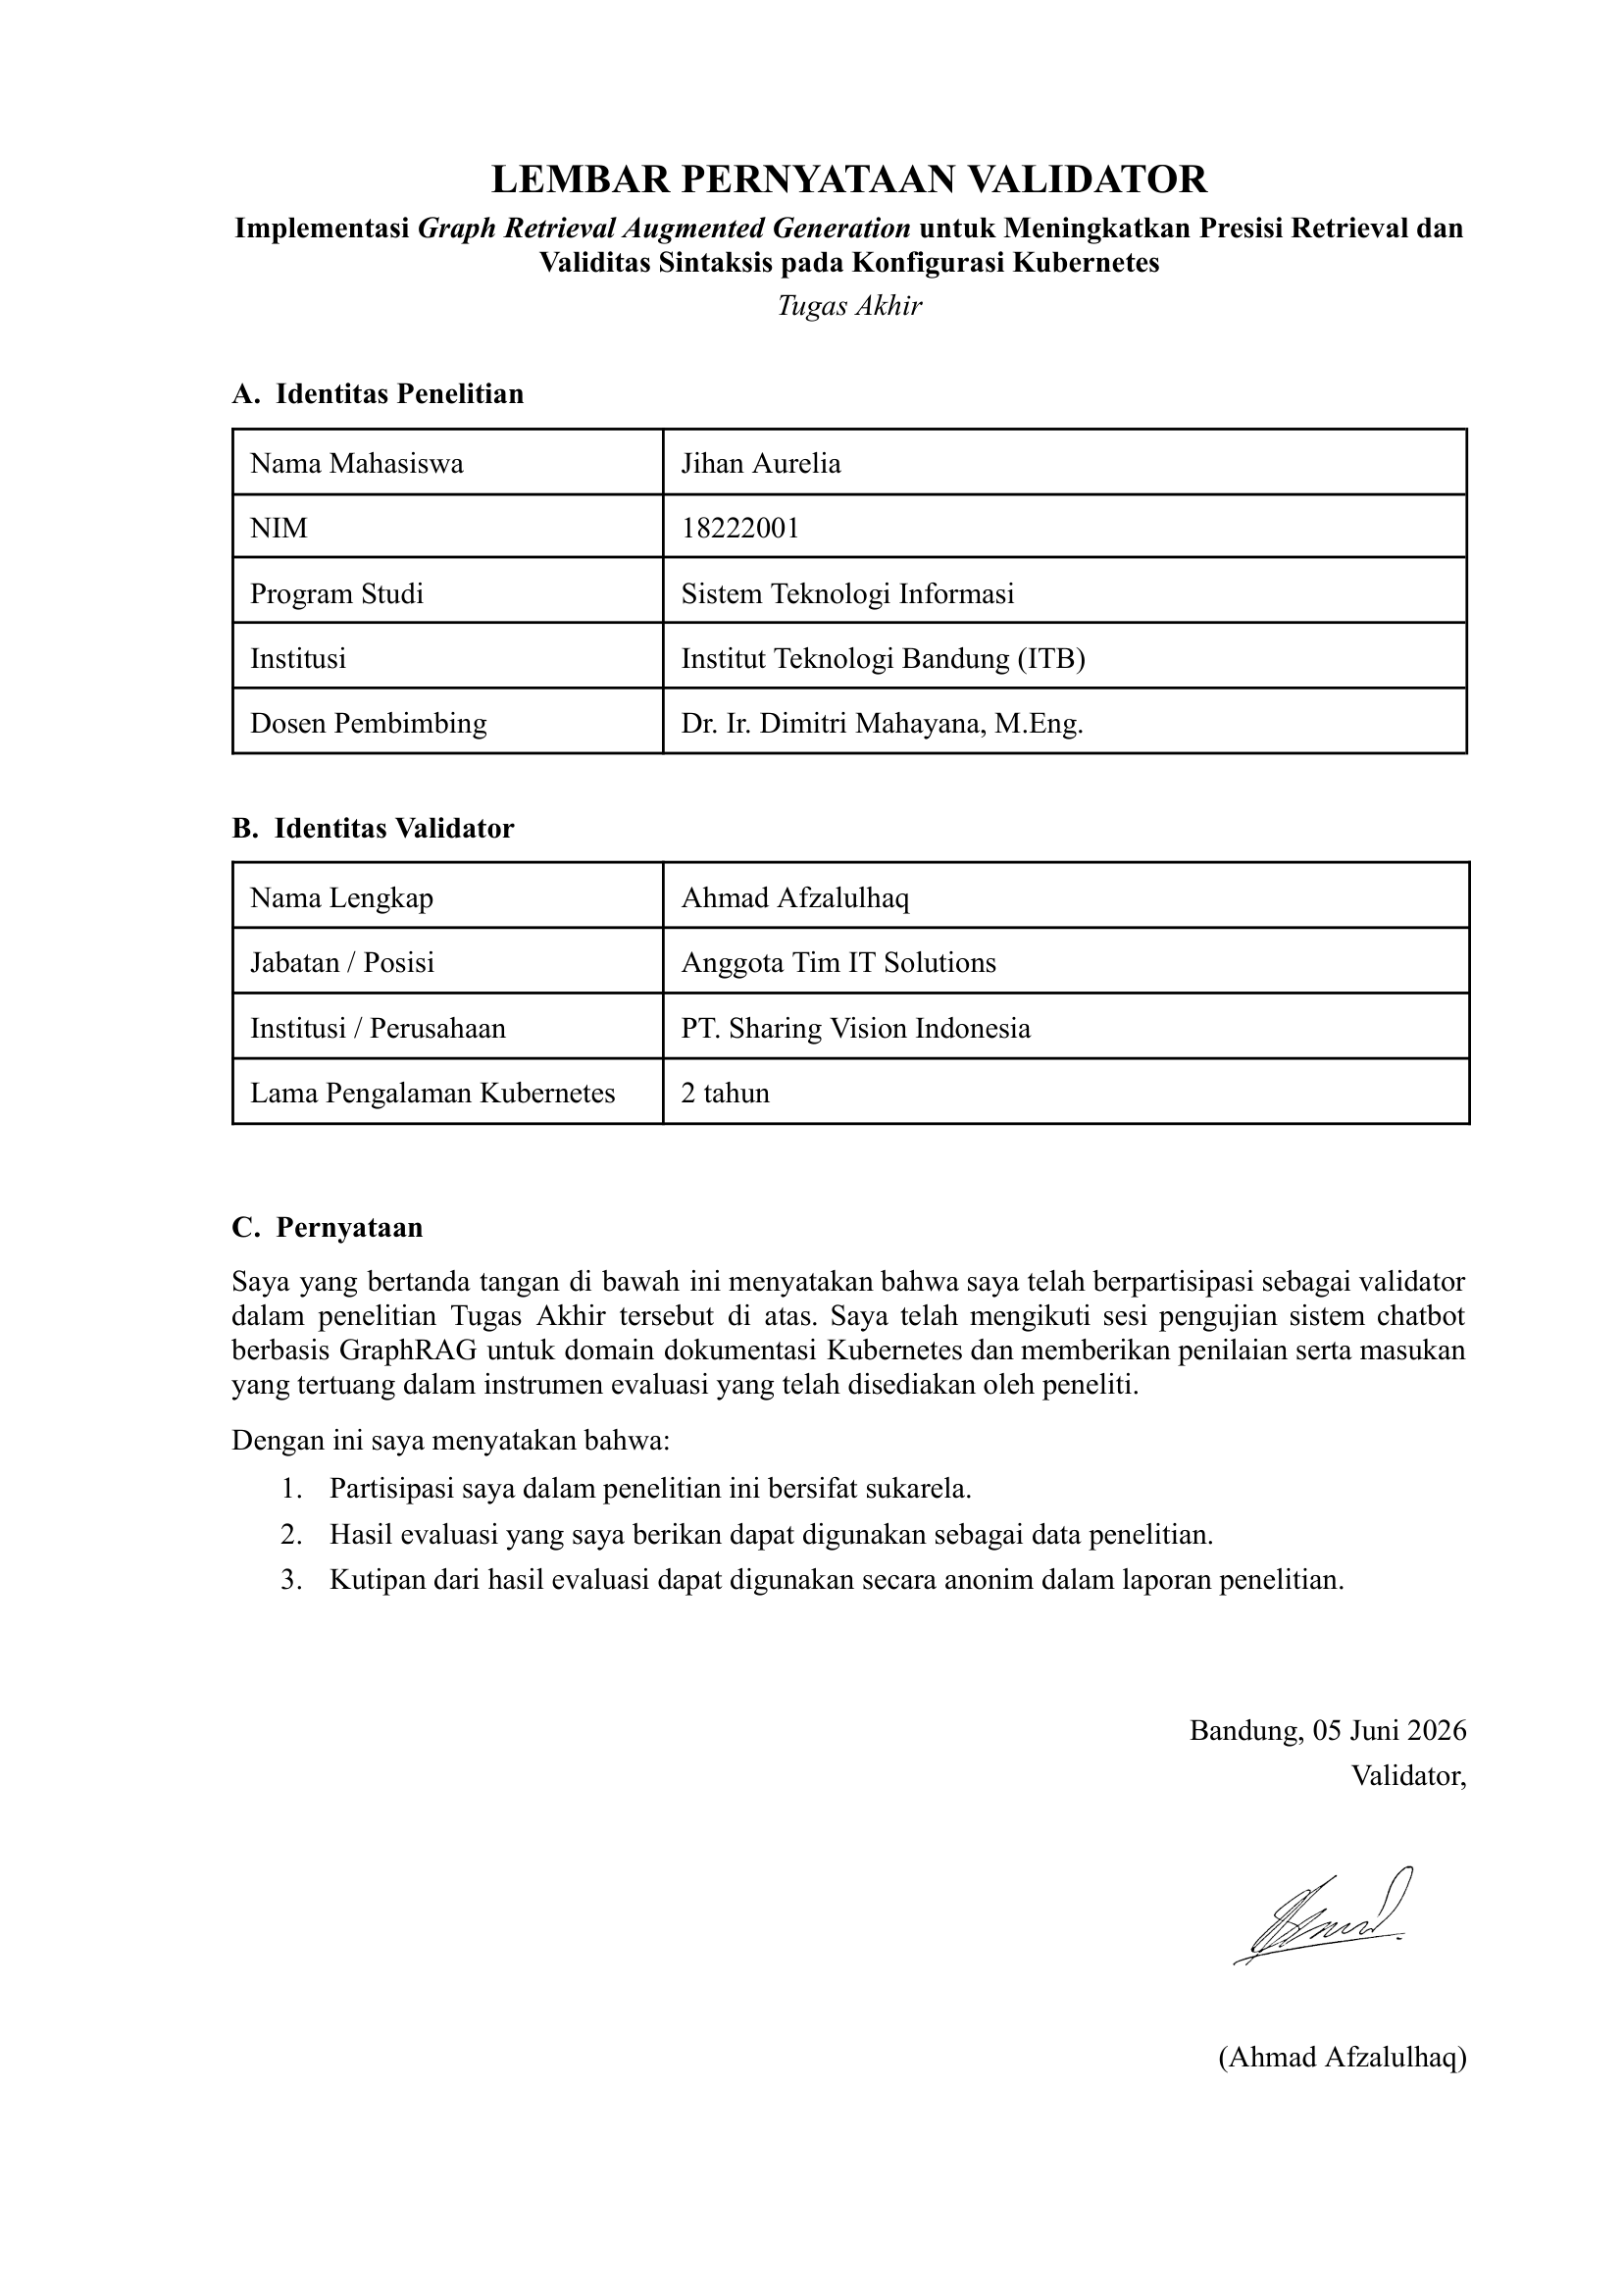
\includegraphics[width=\textwidth, height=0.92\textheight, keepaspectratio]{lampiran-e/ahmad-signed.png}
\end{figure}

\section{Lembar Validasi E.2 --- Raden Dizi Assyafadi}
\begin{figure}[H]
\centering
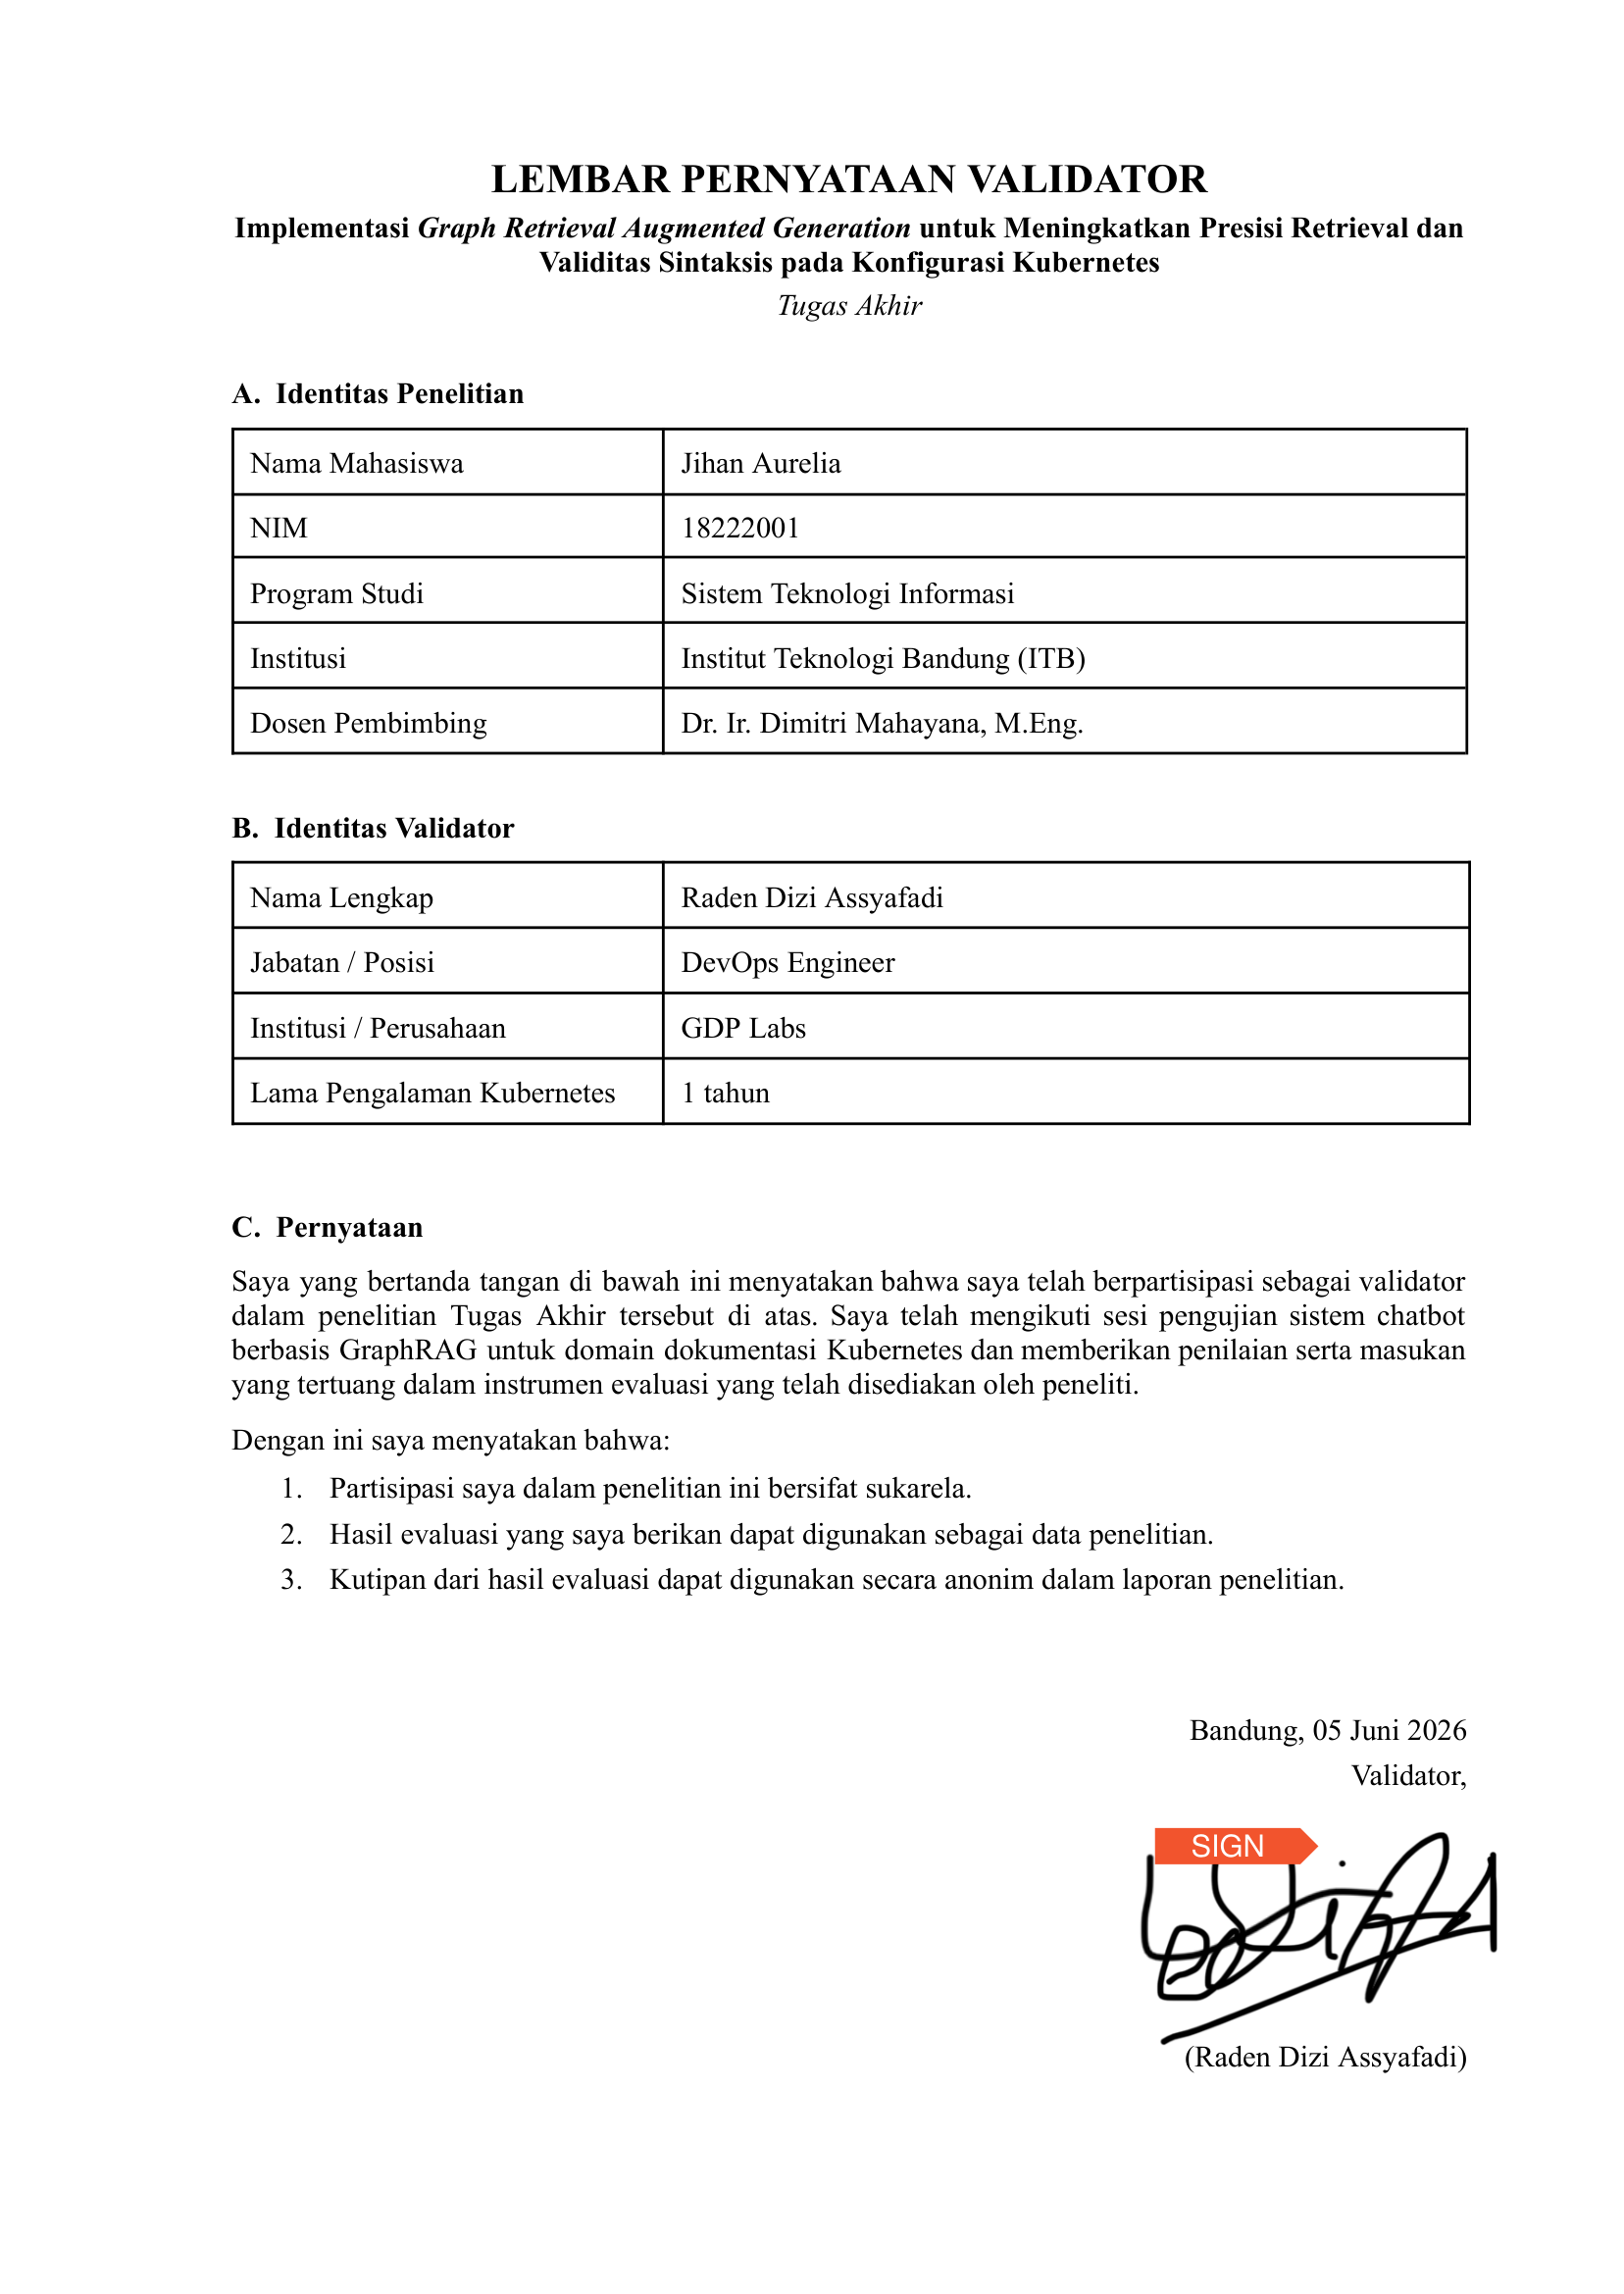
\includegraphics[width=\textwidth, height=0.92\textheight, keepaspectratio]{lampiran-e/raden-signed.png}
\end{figure}

\section{Lembar Validasi E.3 --- Zaky Hassani}
\begin{figure}[H]
\centering
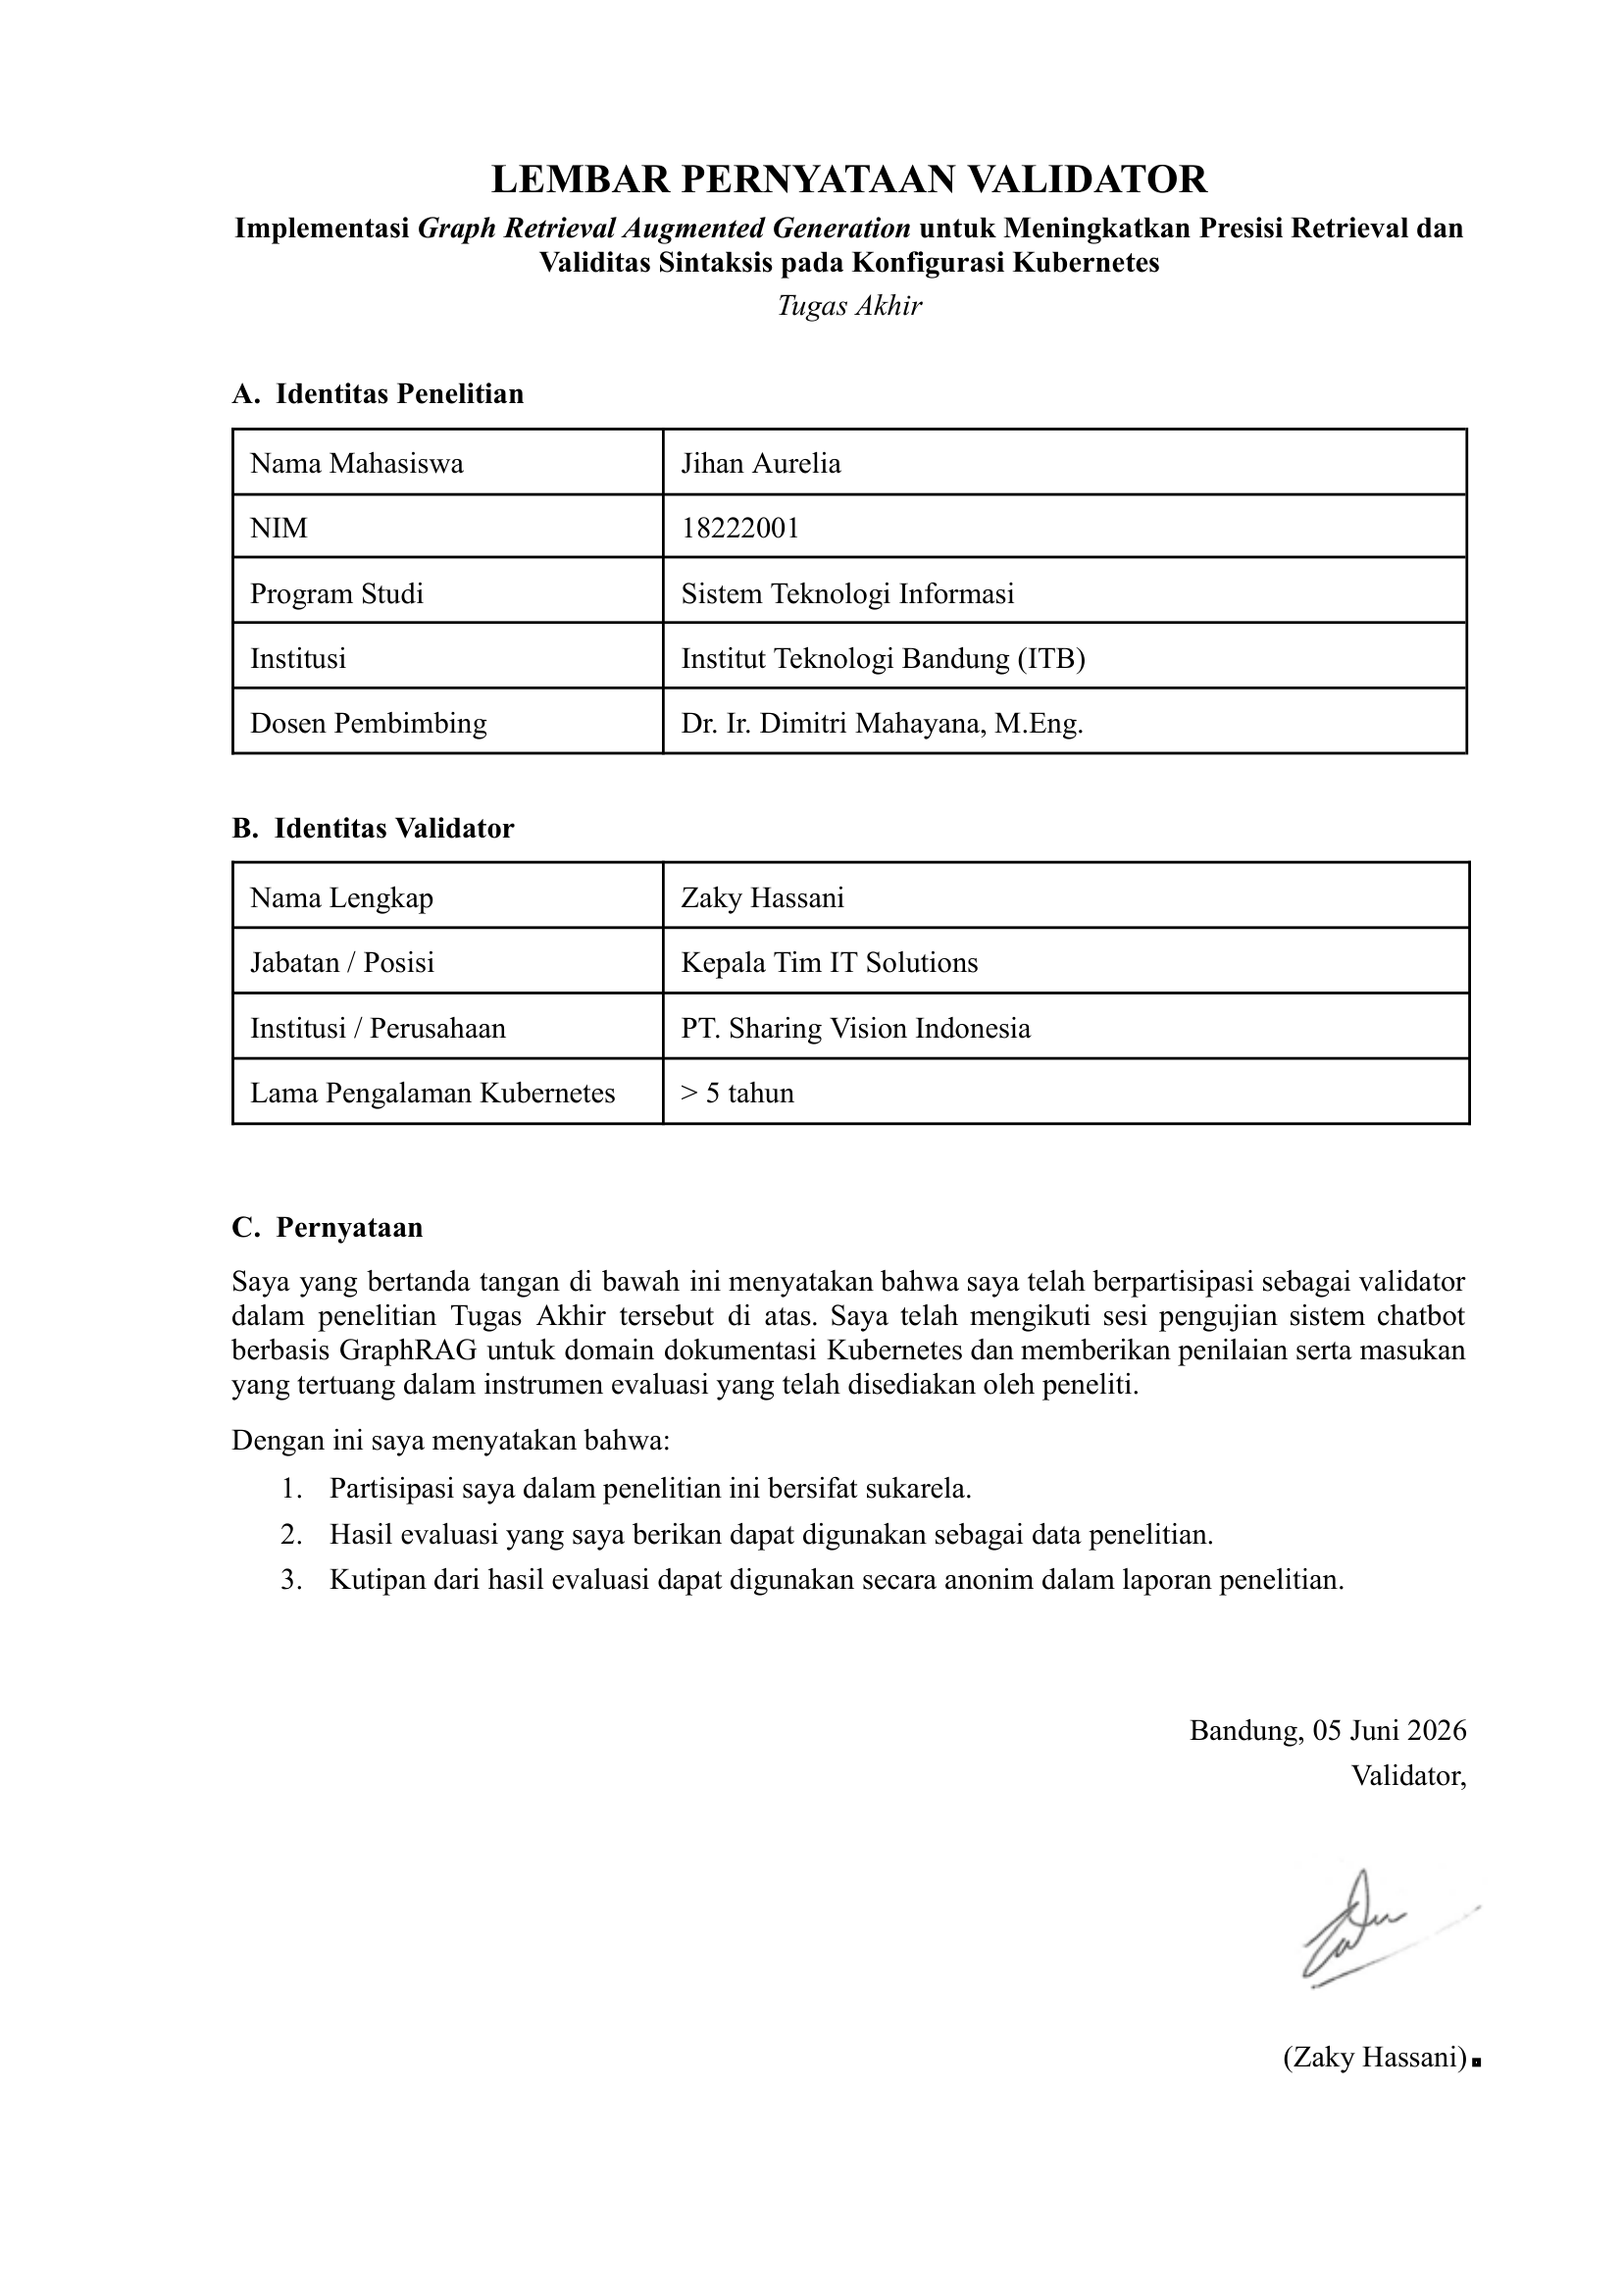
\includegraphics[width=\textwidth, height=0.92\textheight, keepaspectratio]{lampiran-e/zaky-signed.png}
\end{figure}

\section{Lembar Validasi E.4 --- Muhamad Iqbal Ramadhan}
\begin{figure}[H]
\centering
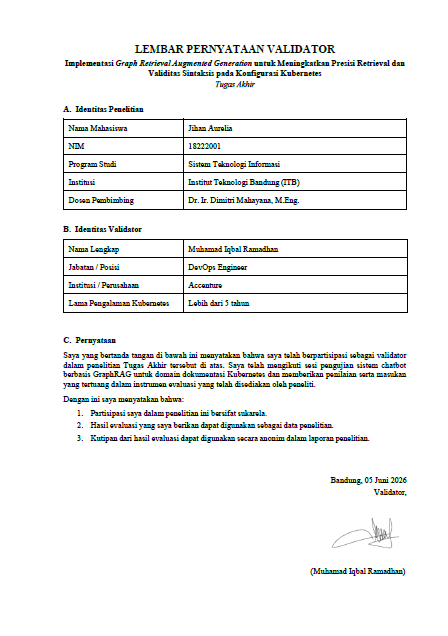
\includegraphics[width=\textwidth, height=0.92\textheight, keepaspectratio]{lampiran-e/iqbal-signed.png}
\end{figure}

\section{Lembar Validasi E.5 --- Muhammad Faiq Dhiya Ul Haq}
\begin{figure}[H]
\centering
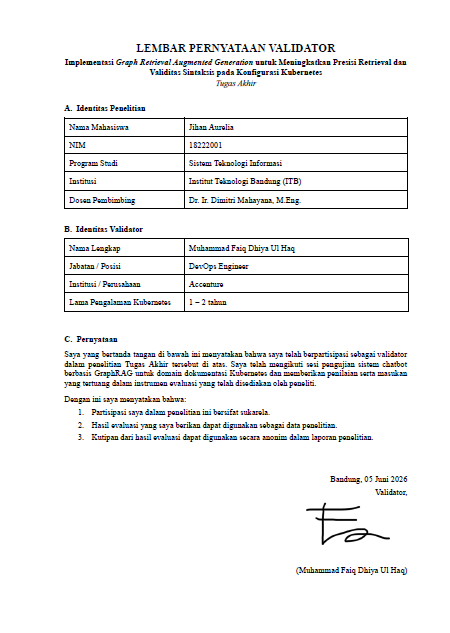
\includegraphics[width=\textwidth, height=0.92\textheight, keepaspectratio]{lampiran-e/faiq-signed.png}
\end{figure}
